\documentclass[Aflevering]{subfiles}
\begin{document}

\subsection{SinusGraf 1 kHz}
\label{app:sinus1000}
\begin{figure}[H]
\centering
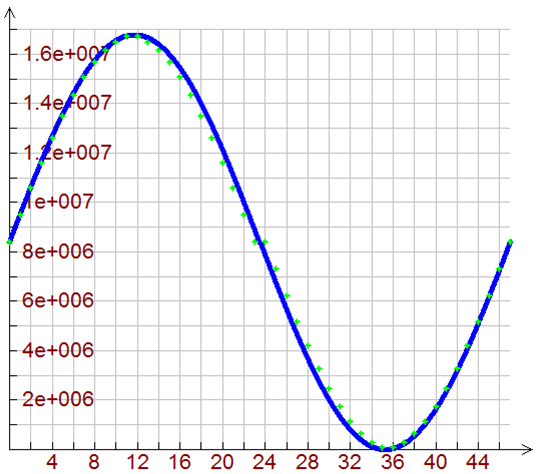
\includegraphics[scale=0.7]{Sine-1-KHz}
\caption{48 samples svarende til en frekvens p� 1000 Hz. Punkterne er output fra vores program og linjen er den �nskede kurve.}
\end{figure}

\subsection{SinusGraf 200 Hz}
\label{app:sinus200}
\begin{figure}[H]
\centering
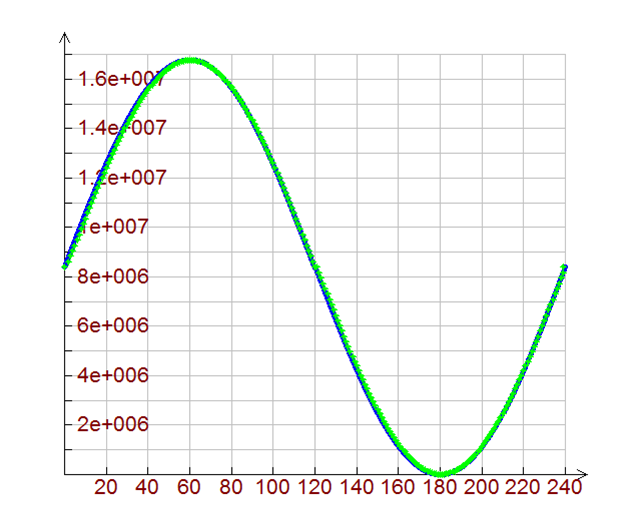
\includegraphics[scale=0.7]{Sine-200Hz}
\caption{240 samples svarende til en frekvens p� 200 Hz. Punkterne er output fra vores program og linjen er den �nskede kurve.}
\end{figure}

\end{document}